\section{Модель SARIMA}

Одной из самых популярных моделей для предсказания временного ряда на сегодняшний день является модель \textit{SARIMA}. Она также реализована в модуле \texttt{statmodels} и представляет собой учитывающее сезонность улучшение модели авторегрессионного интегрированного скользящего среднего. Эта модель предполагает набор параметров для каждой из частей модели: авторегрессионной, интегрированной, скользящего среднего, период сезонности, а также дополнительные термины сезонности. Сначала необходимо провести перебор по этим параметрам, чтобы добиться наиболее стационарного ряда: в таком случае мы сможем предполагать, что будущие характеристики ряда не будут отличаться от нынешних.

После перебора параметров модели мы выбрали те, при которых достигает минимума \textit{информационный критерий Акаике} для данной модели. Этот критерий не только вознаграждает за качество приближения, но и штрафует за излишнее использование параметров модели. Таким образом мы пытаемся избежать переобучения модели. Характеристики получившегося стационарного ряда можно посмотреть на рисунке Рис.~\ref{img:diagn}.

\begin{figure}[h]
        \noindent\centering{
        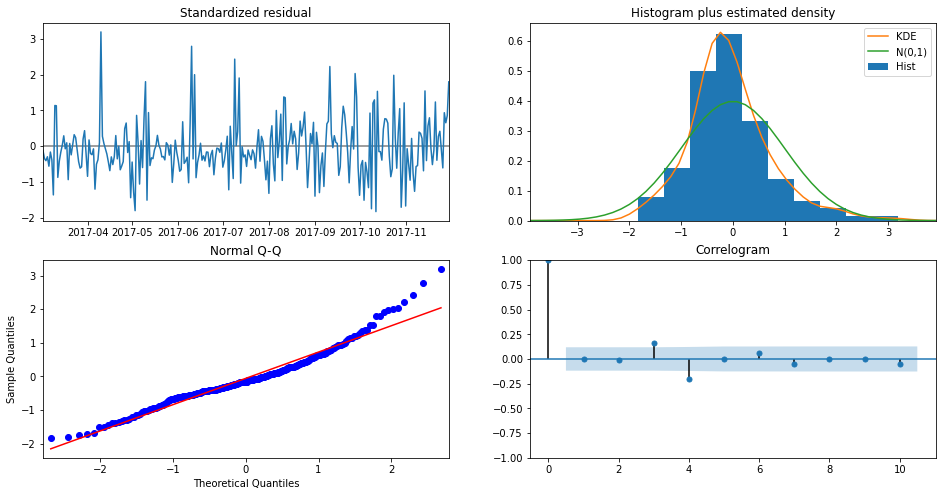
\includegraphics[width=160mm]{content/sarima/diagn.png}
        }
        \caption{Характеристики модели SARIMA с наиболее подходящими параметрами.}
        \label{img:diagn}
\end{figure}

На графике Рис.~\ref{img:pred1} можно визуально оценить точность приближения второго полугодия построенной модели SARIMA, обученной на первом полугодии. На графике Рис.~\ref{img:pred2} видно предсказание на декабрь и дальше. Средняя ошибка за декабрь составляет
$
        72\,340,\!11.
$

\begin{figure}[h]
        \noindent\centering{
        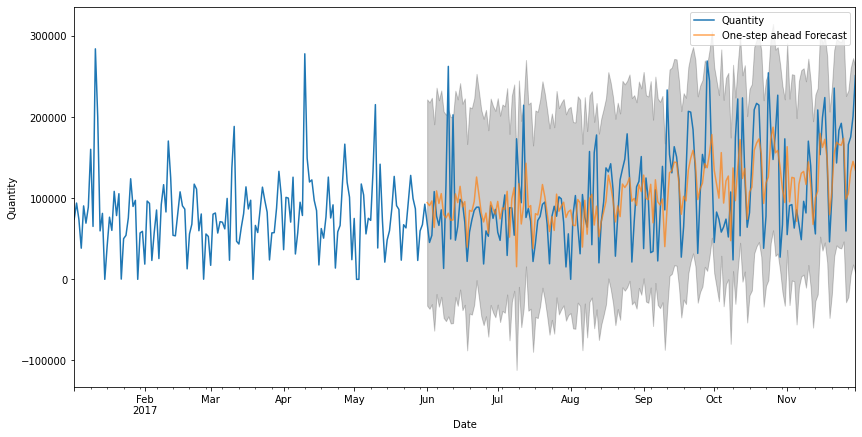
\includegraphics[width=160mm]{content/sarima/pred1.png}
        }
        \caption{Предсказание второго полугодия по первому. Здесь синий --- истинное значение, желтый --- предсказание, серым закрашен доверительный интервал предсказания с уровнем доверия $0,\!05$.}
        \label{img:pred1}
\end{figure}

\begin{figure}[h]
        \noindent\centering{
        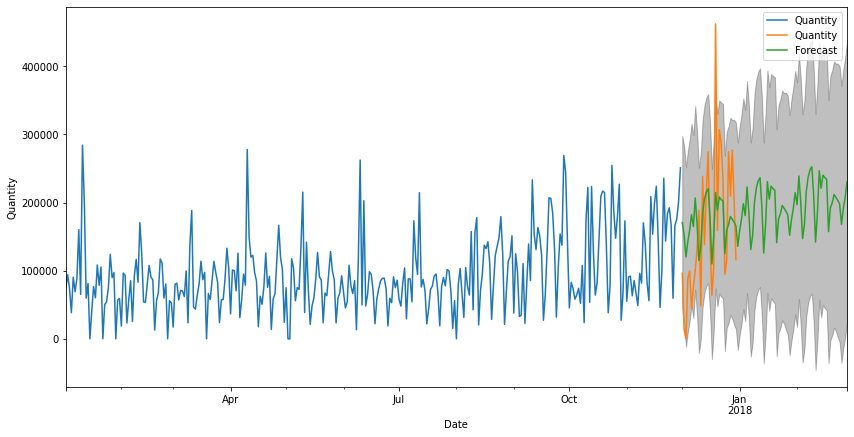
\includegraphics[width=160mm]{content/sarima/pred2.png}
        }
        \caption{Предсказание на 100 дней по 11 месяцам. Здесь синий --- данные, на которых обучалась модель, зеленый --- предсказание модели, желтым --- истинное значение за декабрь (для визуального сравнения), серым закрашен доверительный интервал предсказания с уровнем доверия $0,\!05$.}
        \label{img:pred2}
\end{figure}